\chapter{Les oscillateurs mécaniques}

\textit{Des battements du cœur aux vibrations d'une corde de guitare, en passant par les oscillations d'un véhicule sur ses amortisseurs, les mouvements périodiques sont omniprésents dans la nature et la technique. Ce chapitre étudie les oscillateurs mécaniques, systèmes qui évoluent de façon répétitive autour d'une position d'équilibre. Nous analyserons le pendule élastique (masse-ressort), le pendule simple et le pendule de torsion, en établissant leur équation différentielle caractéristique, leur période propre, et en étudiant les aspects énergétiques. Enfin, nous aborderons les oscillations forcées et le phénomène de résonance, fondamental en ingénierie.}

% ============================================================
\section{Le pendule élastique (masse-ressort)}

\subsection{Système masse-ressort horizontal}

\begin{experience}[Oscillations d'une masse sur un ressort horizontal]
On considère un ressort de masse négligeable, de constante de raideur $k$, fixé à une extrémité. À l'autre extrémité, on accroche une masse $m$ pouvant glisser sans frottement sur une tige horizontale. On écarte la masse de sa position d'équilibre d'une distance $x_m$ et on la lâche sans vitesse initiale. On observe un mouvement de va-et-vient autour de la position d'équilibre $O$.
\end{experience}

\begin{illus}
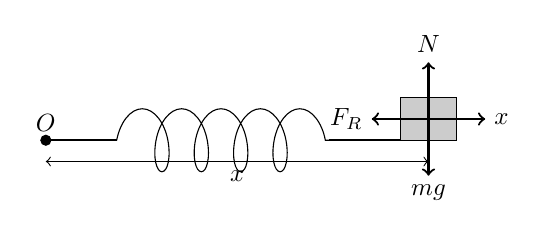
\begin{tikzpicture}[scale=0.9, transform shape]
% Ressort horizontal
\draw[thick] (0,0) -- (1,0);
\draw[decorate, decoration={coil, amplitude=4mm, segment length=5mm}] (1,0) -- (4,0);
\draw[thick] (4,0) -- (5,0);
\filldraw[fill=gray!40] (5,0) rectangle (5.8,0.6);
\draw[->, thick] (5.4,0.3) -- (6.2,0.3) node[right]{$x$};
\draw[dashed] (5.4,0.3) -- (5.4,0);
\draw[->, thick] (5.4,0.3) -- (4.6,0.3) node[left]{$\vect{F}_R$};
\draw[->, thick] (5.4,0.3) -- (5.4,1.1) node[above]{$\vect{N}$};
\draw[->, thick] (5.4,0.3) -- (5.4,-0.5) node[below]{$m\vect{g}$};
\draw[fill=black] (0,0) circle (2pt) node[above]{$O$};
\draw[<->] (0,-0.3) -- (5.4,-0.3) node[midway, below]{$x$};
\end{tikzpicture}
\fig{Schéma du pendule élastique horizontal : masse $m$ sur ressort de raideur $k$.}
\end{illus}

\begin{loi}[Loi de Hooke et équation différentielle]
Dans le domaine élastique, la force de rappel exercée par le ressort est :
\[
\vect{F}_R = -k\,x\,\vect{u}_x
\]
où $x$ est l'écart par rapport à la position d'équilibre. En appliquant la deuxième loi de Newton au système masse-ressort horizontal sans frottement :
\[
m\,\ddot{x} = -k\,x \quad\Longrightarrow\quad \ddot{x} + \frac{k}{m}\,x = 0
\]
On pose $\omega_0^2 = \dfrac{k}{m}$, d'où l'équation différentielle canonique :
\[
\boxed{\ddot{x} + \omega_0^2\,x = 0}
\]
\end{loi}

\begin{definition}[Pulsation propre et période propre]
La pulsation propre $\omega_0$ et la période propre $T_0$ du pendule élastique sont :
\[
\omega_0 = \sqrt{\frac{k}{m}} \qquad ; \qquad T_0 = \frac{2\pi}{\omega_0} = 2\pi\sqrt{\frac{m}{k}}
\]
La fréquence propre est $f_0 = 1/T_0$.
\end{definition}

\begin{propriete}[Solution de l'équation différentielle]
La solution générale de $\ddot{x} + \omega_0^2 x = 0$ s'écrit :
\[
x(t) = X_m\cos(\omega_0 t + \varphi)
\]
où $X_m$ est l'amplitude (en \si{\metre}) et $\varphi$ la phase à l'origine (en \si{\radian}). Les constantes $X_m$ et $\varphi$ sont déterminées par les conditions initiales.
\end{propriete}

\begin{exemple}
Pour un ressort de raideur $k = \SI{20}{\newton\per\metre}$ et une masse $m = \SI{0.5}{\kilogram}$, la période propre est :
\[
T_0 = 2\pi\sqrt{\frac{0.5}{20}} = 2\pi\sqrt{0.025} \approx \SI{0.99}{\second}
\]
\end{exemple}

\subsection{Système masse-ressort vertical}

\begin{experience}[Oscillations verticales]
On suspend verticalement une masse $m$ à un ressort de raideur $k$. À l'équilibre, le ressort est allongé de $\Delta\ell_0 = mg/k$. Si on écarte la masse de cette position d'équilibre et on la lâche, elle oscille verticalement.
\end{experience}

\begin{loi}[Équation différentielle pour le mouvement vertical]
En prenant l'origine $O$ à la position d'équilibre (ressort déjà allongé de $\Delta\ell_0$), la force de rappel totale est $-k\,x$ (où $x$ est l'écart par rapport à $O$). L'équation différentielle est identique au cas horizontal :
\[
\ddot{x} + \frac{k}{m}\,x = 0
\]
La période propre reste $T_0 = 2\pi\sqrt{m/k}$.
\end{loi}

\begin{remarque}
La position d'équilibre verticale est décalée de $\Delta\ell_0$ par rapport à la longueur naturelle du ressort, mais cela n'affecte pas la période des oscillations.
\end{remarque}

% ============================================================
\section{Le pendule simple}

\begin{definition}[Pendule simple]
Un pendule simple est constitué d'une masse ponctuelle $m$ suspendue à un fil inextensible de longueur $\ell$ et de masse négligeable, oscillant dans un plan vertical sous l'effet de la pesanteur.
\end{definition}

\begin{illus}
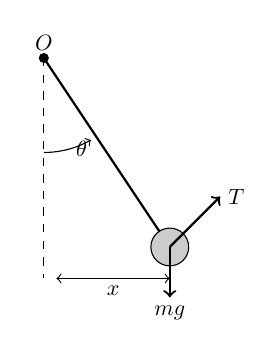
\begin{tikzpicture}[scale=0.8, transform shape]
% Pendule simple
\draw[thick] (0,0) -- (2,-3);
\filldraw[fill=gray!40] (2,-3) circle (0.3);
\draw[->, thick] (2,-3) -- (2,-3.8) node[below]{$m\vect{g}$};
\draw[->, thick] (2,-3) -- (2.8,-2.2) node[right]{$\vect{T}$};
\draw[dashed] (0,0) -- (0,-3.5);
\draw[->] (0,-1.5) arc (270:300:1.5) node[midway, right]{$\theta$};
\draw[fill=black] (0,0) circle (2pt) node[above]{$O$};
\draw[<->] (0.2,-3.5) -- (2,-3.5) node[midway, below]{$x$};
\end{tikzpicture}
\fig{Pendule simple : masse $m$, fil de longueur $\ell$, angle $\theta$.}
\end{illus}

\begin{loi}[Équation différentielle du pendule simple]
Pour de petites oscillations ($\theta \ll \SI{1}{\radian}$), on a $\sin\theta \approx \theta$. Le moment du poids par rapport au point de suspension $O$ est $-mg\ell\sin\theta \approx -mg\ell\,\theta$. Le théorème du moment cinétique donne :
\[
m\ell^2\,\ddot{\theta} = -mg\ell\,\theta \quad\Longrightarrow\quad \ddot{\theta} + \frac{g}{\ell}\,\theta = 0
\]
On pose $\omega_0^2 = g/\ell$, d'où :
\[
\boxed{\ddot{\theta} + \omega_0^2\,\theta = 0}
\]
\end{loi}

\begin{definition}[Période propre du pendule simple]
La période propre pour les petites oscillations est :
\[
T_0 = 2\pi\sqrt{\frac{\ell}{g}}
\]
Elle ne dépend ni de la masse $m$, ni de l'amplitude (isochronisme des petites oscillations).
\end{definition}

\begin{exemple}
Un pendule de longueur $\ell = \SI{1.0}{\metre}$ à Yaoundé ($g = \SI{9.78}{\metre\per\second\squared}$) a une période :
\[
T_0 = 2\pi\sqrt{\frac{1.0}{9.78}} \approx \SI{2.01}{\second}
\]
\end{exemple}

% ============================================================
\section{Le pendule de torsion}

\begin{definition}[Pendule de torsion]
Un pendule de torsion est constitué d'un fil (ou d'une tige) élastique de constante de torsion $C$, fixé à une extrémité, et portant à l'autre extrémité un solide de moment d'inertie $J$ par rapport à l'axe du fil. Lorsqu'on tord le fil d'un angle $\theta$, il exerce un couple de rappel $\mathcal{M} = -C\,\theta$.
\end{definition}

\begin{illus}
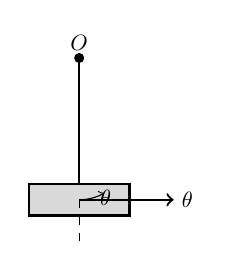
\begin{tikzpicture}[scale=0.8, transform shape]
% Pendule de torsion
\draw[thick] (0,0) -- (0,-2);
\draw[thick, fill=gray!30] (-0.8,-2) rectangle (0.8,-2.5);
\draw[->, thick] (0,-2.25) -- (1.5,-2.25) node[right]{$\theta$};
\draw[dashed] (0,-2.25) -- (0,-3);
\draw[->] (0,-2.25) arc (270:300:0.8) node[midway, right]{$\theta$};
\draw[fill=black] (0,0) circle (2pt) node[above]{$O$};
\end{tikzpicture}
\fig{Pendule de torsion : fil de constante $C$, moment d'inertie $J$.}
\end{illus}

\begin{loi}[Équation différentielle du pendule de torsion]
Le théorème du moment cinétique appliqué au solide donne :
\[
J\,\ddot{\theta} = -C\,\theta \quad\Longrightarrow\quad \ddot{\theta} + \frac{C}{J}\,\theta = 0
\]
On pose $\omega_0^2 = C/J$, d'où :
\[
\boxed{\ddot{\theta} + \omega_0^2\,\theta = 0}
\]
La période propre est $T_0 = 2\pi\sqrt{J/C}$.
\end{loi}

\begin{remarque}
Le pendule de torsion est utilisé dans les horloges mécaniques et les galvanomètres à cadre mobile.
\end{remarque}

% ============================================================
\section{Énergie mécanique de l'oscillateur harmonique}

\subsection{Cas du pendule élastique}

\begin{propriete}[Énergie mécanique]
Pour un oscillateur harmonique non amorti (masse-ressort), l'énergie mécanique $E_m$ est constante :
\[
E_m = E_c + E_p = \frac{1}{2}m\dot{x}^2 + \frac{1}{2}k x^2 = \frac{1}{2}k X_m^2 = \text{constante}
\]
où $X_m$ est l'amplitude du mouvement.
\end{propriete}

\begin{illus}
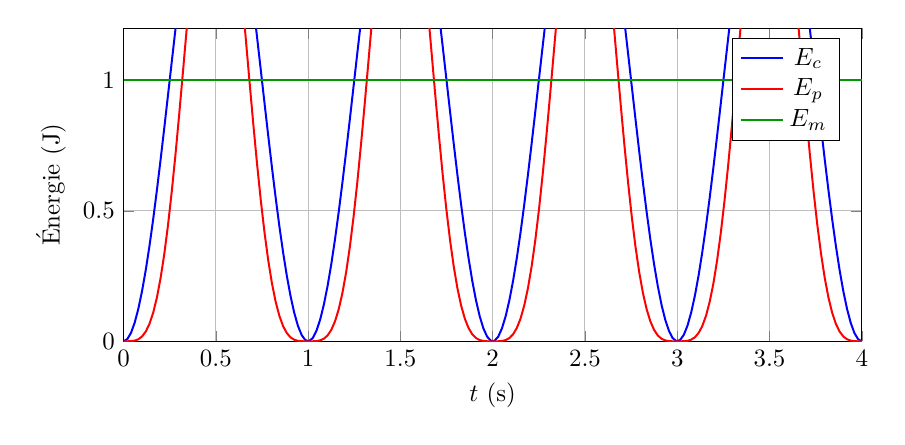
\begin{tikzpicture}[scale=0.9]
\begin{axis}[
    xlabel={$t$ (s)},
    ylabel={Énergie (J)},
    xmin=0, xmax=4,
    ymin=0, ymax=1.2,
    legend pos=north east,
    grid=both,
    width=12cm,
    height=6cm
]
\addplot[domain=0:4, samples=200, thick, blue] {0.5*(1 - cos(deg(2*pi*x)))^2 + 0.5*(sin(deg(2*pi*x)))^2};
\addlegendentry{$E_c$}
\addplot[domain=0:4, samples=200, thick, red] {0.5*(1 - cos(deg(2*pi*x)))^2};
\addlegendentry{$E_p$}
\addplot[domain=0:4, samples=200, thick, green!60!black] {1};
\addlegendentry{$E_m$}
\end{axis}
\end{tikzpicture}
\fig{Évolution temporelle des énergies cinétique $E_c$, potentielle $E_p$ et mécanique $E_m$ pour un oscillateur harmonique.}
\end{illus}

\begin{aretenir}
Dans un oscillateur harmonique non amorti, l'énergie mécanique se conserve : il y a échange permanent entre énergie cinétique et énergie potentielle.
\end{aretenir}

\subsection{Amortissement}

\begin{definition}[Oscillations amorties]
En présence de frottements (visqueux, solides), l'énergie mécanique diminue au cours du temps : l'amplitude des oscillations décroît exponentiellement. On parle d'oscillations amorties.
\end{definition}

\begin{remarque}
Si l'amortissement est trop fort (amortissement critique ou sur-critique), le système ne peut plus osciller et retourne à l'équilibre sans dépassement.
\end{remarque}

% ============================================================
\section{Oscillations forcées et résonance}

\begin{experience}[Oscillations forcées]
On soumet un oscillateur mécanique (masse-ressort, pendule) à une excitation sinusoïdale de fréquence $f$ (par exemple via un moteur excentrique). On observe que l'amplitude des oscillations dépend de la fréquence de l'excitation.
\end{experience}

\begin{definition}[Résonance]
La résonance mécanique se produit lorsque la fréquence de l'excitation $f$ est égale à la fréquence propre $f_0$ de l'oscillateur. L'amplitude des oscillations est alors maximale.
\end{definition}

\begin{illus}
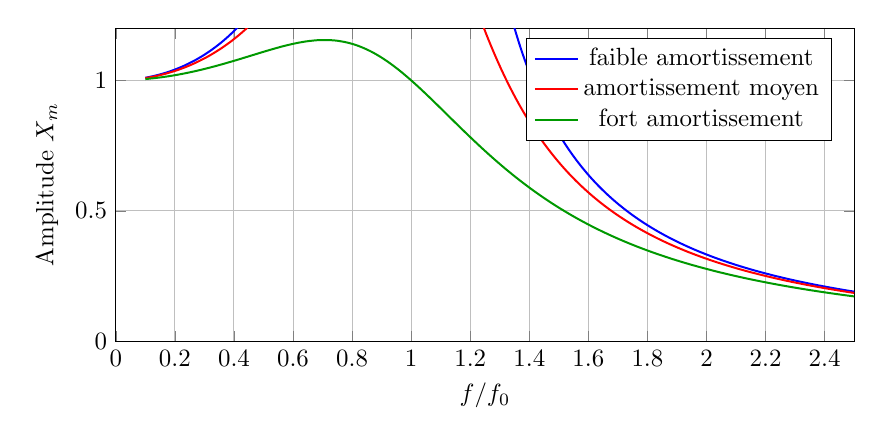
\begin{tikzpicture}[scale=0.9]
\begin{axis}[
    xlabel={$f/f_0$},
    ylabel={Amplitude $X_m$},
    xmin=0, xmax=2.5,
    ymin=0, ymax=1.2,
    legend pos=north east,
    grid=both,
    width=12cm,
    height=6cm
]
\addplot[domain=0.1:2.5, samples=200, thick, blue] {1/sqrt((1 - x^2)^2 + (0.1*x)^2)};
\addlegendentry{faible amortissement}
\addplot[domain=0.1:2.5, samples=200, thick, red] {1/sqrt((1 - x^2)^2 + (0.5*x)^2)};
\addlegendentry{amortissement moyen}
\addplot[domain=0.1:2.5, samples=200, thick, green!60!black] {1/sqrt((1 - x^2)^2 + (1.0*x)^2)};
\addlegendentry{fort amortissement}
\end{axis}
\end{tikzpicture}
\fig{Courbes de résonance d'un oscillateur forcé pour différents amortissements.}
\end{illus}

\begin{aretenir}
\begin{itemize}
    \item À la résonance, l'amplitude est maximale et le déphasage entre l'excitation et la réponse est de $\pi/2$.
    \item Plus l'amortissement est faible, plus la résonance est aiguë (amplitude élevée et pic étroit).
    \item La résonance peut être destructive (ex. : pont qui s'effondre sous l'effet du vent).
\end{itemize}
\end{aretenir}

% ============================================================
\section{L'essentiel à retenir}

\begin{synthese}
\paragraph{Lois fondamentales}
\begin{itemize}
    \item Équation différentielle de l'oscillateur harmonique : $\ddot{x} + \omega_0^2 x = 0$
    \item Solution : $x(t) = X_m\cos(\omega_0 t + \varphi)$
\end{itemize}

\paragraph{Périodes propres}
\begin{itemize}
    \item Pendule élastique (masse-ressort) : $T_0 = 2\pi\sqrt{m/k}$
    \item Pendule simple (petites oscillations) : $T_0 = 2\pi\sqrt{\ell/g}$
    \item Pendule de torsion : $T_0 = 2\pi\sqrt{J/C}$
\end{itemize}

\paragraph{Énergie}
\begin{itemize}
    \item Oscillateur non amorti : $E_m = \frac{1}{2}k X_m^2 = \text{constante}$
    \item Oscillateur amorti : $E_m$ diminue, amplitude décroît exponentiellement
\end{itemize}

\paragraph{Résonance}
\begin{itemize}
    \item $f_{\text{exc}} = f_0$ $\Rightarrow$ amplitude maximale
    \item Déphasage de $\pi/2$ à la résonance
    \item Amortissement faible $\Rightarrow$ résonance aiguë
\end{itemize}

\paragraph{Unités}
\begin{itemize}
    \item $k$ : \si{\newton\per\metre} ; $m$ : \si{\kilogram} ; $\ell$ : \si{\metre}
    \item $T_0$ : \si{\second} ; $f_0$ : \si{\hertz} ; $\omega_0$ : \si{\radian\per\second}
    \item $C$ : \si{\newton\metre\per\radian} ; $J$ : \si{\kilogram\metre\squared}
\end{itemize}

\paragraph{Attention aux pièges}
\begin{itemize}
    \item Ne pas confondre pulsation $\omega_0$ et fréquence $f_0$ : $\omega_0 = 2\pi f_0$
    \item Le pendule simple n'est harmonique que pour $\theta \ll \SI{1}{\radian}$
    \item L'énergie mécanique n'est constante qu'en l'absence de frottements
\end{itemize}
\end{synthese}

% ============================================================
\section{Méthodes \& savoir-faire}

\methode{Déterminer la période propre d'un oscillateur}
Pour un oscillateur donné, identifier le type (masse-ressort, pendule simple, torsion), relever les paramètres ($m$, $k$, $\ell$, $g$, $J$, $C$) et appliquer la formule appropriée. Vérifier les unités.

\begin{exemple}
Un ressort de raideur $k = \SI{40}{\newton\per\metre}$ supporte une masse $m = \SI{200}{\gram}$. Calculer $T_0$.
\corrige{de l'exemple}
$T_0 = 2\pi\sqrt{m/k} = 2\pi\sqrt{0.200/40} = 2\pi\sqrt{0.005} \approx \SI{0.444}{\second}$.
\end{exemple}

\methode{Établir l'équation différentielle d'un oscillateur}
Appliquer la deuxième loi de Newton (ou le théorème du moment cinétique) au système. Exprimer la force de rappel (ou le couple de rappel) en fonction de l'écart à l'équilibre. Simplifier pour obtenir $\ddot{x} + \omega_0^2 x = 0$.

\begin{exemple}
Pour un pendule simple, le moment du poids est $-mg\ell\sin\theta$. Pour $\theta$ petit, $\sin\theta \approx \theta$, d'où $m\ell^2\ddot{\theta} = -mg\ell\theta$ $\Rightarrow$ $\ddot{\theta} + (g/\ell)\theta = 0$.
\end{exemple}

\methode{Utiliser les conditions initiales}
Les conditions initiales $x(0)$ et $\dot{x}(0)$ permettent de déterminer $X_m$ et $\varphi$ dans $x(t) = X_m\cos(\omega_0 t + \varphi)$.

\begin{exemple}
Si $x(0) = X_0$ et $\dot{x}(0) = 0$, alors $X_m = X_0$ et $\varphi = 0$.
\end{exemple}

\methode{Calculer l'énergie mécanique}
Pour un oscillateur harmonique, $E_m = \frac{1}{2}k X_m^2$. Utiliser la conservation de l'énergie pour relier vitesse et position.

\begin{exemple}
Une masse $m = \SI{0.1}{\kilogram}$ oscille avec $X_m = \SI{0.05}{\metre}$ et $k = \SI{10}{\newton\per\metre}$. $E_m = \frac{1}{2} \times 10 \times (0.05)^2 = \SI{0.0125}{\joule}$.
\end{exemple}

\methode{Analyser la résonance}
Identifier la fréquence propre $f_0$ de l'oscillateur. La résonance a lieu quand $f_{\text{exc}} = f_0$. L'amplitude est maximale et le déphasage vaut $\pi/2$.

\begin{exemple}
Un moteur tourne à $\num{1200}~\mathrm{tr/min}$ ($f = \SI{20}{\hertz}$). Pour qu'il y ait résonance avec un ressort de $k = \SI{100}{\newton\per\metre}$, il faut $m = k/(4\pi^2 f^2) \approx \SI{0.0063}{\kilogram}$.
\end{exemple}

\methode{Distinguer oscillations libres, amorties et forcées}
\begin{itemize}
    \item Oscillations libres : pas d'excitation extérieure, $f = f_0$.
    \item Oscillations amorties : présence de frottements, amplitude décroît.
    \item Oscillations forcées : excitation sinusoïdale extérieure, fréquence imposée.
\end{itemize}

% ============================================================
\section{Exercices d'application}

\rubrique{Pendule élastique}

\exo{}\diff{1} Un ressort de raideur $k = \SI{50}{\newton\per\metre}$ est comprimé de $\SI{0.1}{\metre}$ par une masse $m = \SI{0.2}{\kilogram}$ posée dessus. On lâche le système. Calculer la période propre et l'énergie mécanique initiale.

\exo{}\diff{2} Une masse $m = \SI{0.5}{\kilogram}$ est attachée à un ressort vertical de $k = \SI{20}{\newton\per\metre}$. Déterminer l'allongement à l'équilibre et la période des oscillations verticales.

\exo{}\diff{2} Un oscillateur masse-ressort a une période $T_0 = \SI{0.5}{\second}$ pour $m = \SI{0.1}{\kilogram}$. Quelle est la raideur $k$ du ressort ?

\rubrique{Pendule simple}

\exo{}\diff{1} Un pendule simple de longueur $\ell = \SI{0.8}{\metre}$ oscille à Douala ($g = \SI{9.79}{\metre\per\second\squared}$). Calculer sa période propre.

\exo{}\diff{2} On veut qu'un pendule simple ait une période de $\SI{2.0}{\second}$. Quelle doit être sa longueur ? (Prendre $g = \SI{9.8}{\metre\per\second\squared}$)

\exo{}\diff{3} Un pendule simple bat la seconde à Paris ($g = \SI{9.81}{\metre\per\second\squared}$). Quelle serait sa période à Yaoundé ($g = \SI{9.78}{\metre\per\second\squared}$) ?

\rubrique{Pendule de torsion}

\exo{}\diff{1} Un fil de torsion a une constante $C = \SI{0.01}{\newton\metre\per\radian}$. On y suspend un disque de moment d'inertie $J = \SI{0.002}{\kilogram\metre\squared}$. Calculer la période propre.

\exo{}\diff{2} Un pendule de torsion a une période $T_0 = \SI{1.5}{\second}$ pour $J = \SI{0.005}{\kilogram\metre\squared}$. Déterminer $C$.

\rubrique{Énergie mécanique}

\exo{}\diff{2} Un oscillateur masse-ressort a $k = \SI{100}{\newton\per\metre}$ et $X_m = \SI{0.02}{\metre}$. Calculer l'énergie mécanique et la vitesse maximale de la masse $m = \SI{0.1}{\kilogram}$.

\exo{}\diff{2} À $t = 0$, $x = \SI{0.01}{\metre}$ et $\dot{x} = \SI{0.2}{\metre\per\second}$ pour $m = \SI{0.05}{\kilogram}$ et $k = \SI{20}{\newton\per\metre}$. Déterminer $X_m$ et $\varphi$.

\rubrique{Résonance}

\exo{}\diff{2} Un oscillateur de $f_0 = \SI{10}{\hertz}$ est excité par une force sinusoïdale. À quelle fréquence se produit la résonance ? Que vaut le déphasage à cette fréquence ?

\exo{}\diff{3} Un moteur tournant à $\num{1500}~\mathrm{tr/min}$ provoque des vibrations sur un support de raideur $k = \SI{5000}{\newton\per\metre}$. Quelle masse doit avoir le support pour éviter la résonance ?

% ============================================================
\section{Exercices d'entraînement}

\rubrique{Pendule élastique}

\exo{}\diff{2} Un ressort de $k = \SI{30}{\newton\per\metre}$ supporte une masse $m = \SI{0.3}{\kilogram}$. On écarte la masse de $\SI{0.05}{\metre}$ et on la lâche. Écrire $x(t)$.

\exo{}\diff{2} Deux ressorts identiques de $k = \SI{15}{\newton\per\metre}$ sont montés en parallèle. Quelle est la raideur équivalente ? Si on y accroche $m = \SI{0.2}{\kilogram}$, quelle est $T_0$ ?

\exo{}\diff{3} Un ressort de $k = \SI{40}{\newton\per\metre}$ et $m = \SI{0.1}{\kilogram}$ oscille avec une amplitude $X_m = \SI{0.03}{\metre}$. Calculer la vitesse lorsque $x = \SI{0.015}{\metre}$.

\rubrique{Pendule simple}

\exo{}\diff{1} Un pendule simple de $\ell = \SI{1.2}{\metre}$ a-t-il une période plus grande ou plus petite qu'un pendule de $\ell = \SI{0.6}{\metre}$ ? Justifier.

\exo{}\diff{2} Un pendule simple bat la seconde ($T_0 = \SI{2}{\second}$) à un lieu où $g = \SI{9.8}{\metre\per\second\squared}$. Quelle est sa longueur ?

\exo{}\diff{3} On double la longueur d'un pendule simple. Par quel facteur est multipliée sa période ?

\rubrique{Pendule de torsion}

\exo{}\diff{2} Un pendule de torsion a $C = \SI{0.02}{\newton\metre\per\radian}$ et $J = \SI{0.004}{\kilogram\metre\squared}$. On le tord de $\ang{30}$ et on le lâche. Écrire $\theta(t)$.

\exo{}\diff{3} On triple le moment d'inertie d'un pendule de torsion. Comment change sa période ?

\rubrique{Énergie et amortissement}

\exo{}\diff{2} Un oscillateur amorti a une amplitude qui décroît de $\SI{10}{\percent}$ par période. Quel pourcentage de l'énergie mécanique est perdu par période ?

\exo{}\diff{3} Un oscillateur de $m = \SI{0.2}{\kilogram}$ et $k = \SI{80}{\newton\per\metre}$ a une amplitude initiale $X_0 = \SI{0.04}{\metre}$. Après 5 périodes, l'amplitude est $X_5 = \SI{0.02}{\metre}$. Calculer le coefficient d'amortissement.

\rubrique{Résonance}

\exo{}\diff{2} Un pont a une fréquence propre $f_0 = \SI{1.2}{\hertz}$. Le vent provoque des oscillations forcées à $f = \SI{1.2}{\hertz}$. Que risque-t-il de se produire ?

\exo{}\diff{3} Un oscillateur forcé a un amortissement faible. Décrire qualitativement l'allure de la courbe d'amplitude en fonction de la fréquence.

\rubrique{Problèmes ouverts}

\exo{}\diff{3} Un ressort de $k = \SI{25}{\newton\per\metre}$ est comprimé de $\SI{0.08}{\metre}$ par une masse $m = \SI{0.15}{\kilogram}$. On lâche. Déterminer $x(t)$, $v(t)$, $E_c(t)$, $E_p(t)$ et $E_m$.

\exo{}\diff{3} Un pendule simple de $\ell = \SI{0.5}{\metre}$ est écarté de $\ang{10}$ et lâché. Calculer sa vitesse au passage à la verticale (utiliser la conservation de l'énergie).

% ============================================================
\section{Sujets type Baccalauréat}

\sujetbac[Oscillateur masse-ressort horizontal]
\begin{enumerate}[label=\arabic*)]
    \item Un ressort de raideur $k = \SI{20}{\newton\per\metre}$ est fixé à un mur. À son extrémité libre, on accroche une masse $m = \SI{0.4}{\kilogram}$ pouvant glisser sans frottement sur une table horizontale.
    \begin{enumerate}[label=\alph*)]
        \item Établir l'équation différentielle du mouvement.
        \item Calculer la période propre $T_0$.
        \item À $t=0$, on écarte la masse de $\SI{0.05}{\metre}$ vers la droite et on la lâche sans vitesse. Déterminer $x(t)$.
    \end{enumerate}
    \item On ajoute un amortisseur visqueux de coefficient $b = \SI{0.5}{\newton\second\per\metre}$.
    \begin{enumerate}[label=\alph*)]
        \item Écrire la nouvelle équation différentielle.
        \item Montrer que le mouvement est pseudo-périodique et calculer la pseudo-période.
    \end{enumerate}
    \item On supprime l'amortisseur et on soumet la masse à une force excitatrice $F(t) = F_0\cos(2\pi f t)$ avec $F_0 = \SI{1}{\newton}$.
    \begin{enumerate}[label=\alph*)]
        \item Pour quelle fréquence $f$ observe-t-on la résonance ?
        \item Que vaut l'amplitude à la résonance si l'amortissement résiduel est négligeable ?
    \end{enumerate}
\end{enumerate}

\sujetbac[Pendule simple et horloge]
\begin{enumerate}[label=\arabic*)]
    \item Un pendule simple de longueur $\ell = \SI{1.0}{\metre}$ est utilisé comme balancier d'une horloge.
    \begin{enumerate}[label=\alph*)]
        \item Rappeler l'expression de la période propre $T_0$ d'un pendule simple.
        \item Calculer $T_0$ à Douala ($g = \SI{9.79}{\metre\per\second\squared}$).
        \item L'horloge avance-t-elle ou retarde-t-elle si on la transporte à Yaoundé ($g = \SI{9.78}{\metre\per\second\squared}$) ? Justifier.
    \end{enumerate}
    \item Pour régler l'horloge, on modifie la longueur du pendule.
    \begin{enumerate}[label=\alph*)]
        \item Quelle doit être la nouvelle longueur $\ell'$ pour que $T_0 = \SI{2.00}{\second}$ à Yaoundé ?
        \item De combien faut-il modifier la longueur ?
    \end{enumerate}
    \item Le pendule est écarté de $\ang{5}$ de sa position d'équilibre et lâché.
    \begin{enumerate}[label=\alph*)]
        \item Calculer l'énergie mécanique du pendule (masse $m = \SI{0.1}{\kilogram}$).
        \item En déduire la vitesse maximale de la masse.
    \end{enumerate}
\end{enumerate}

\sujetbac[Pendule de torsion et moment d'inertie]
\begin{enumerate}[label=\arabic*)]
    \item Un fil de torsion de constante $C = \SI{0.015}{\newton\metre\per\radian}$ est fixé à un support. On y suspend un disque de moment d'inertie $J$ inconnu.
    \begin{enumerate}[label=\alph*)]
        \item Établir l'équation différentielle du mouvement de torsion.
        \item La période mesurée est $T_0 = \SI{1.2}{\second}$. Calculer $J$.
    \end{enumerate}
    \item On ajoute une masse ponctuelle $m = \SI{0.05}{\kilogram}$ à une distance $d = \SI{0.1}{\metre}$ de l'axe.
    \begin{enumerate}[label=\alph*)]
        \item Quel est le nouveau moment d'inertie $J'$ ?
        \item Calculer la nouvelle période $T_0'$.
    \end{enumerate}
    \item Le fil est tordu de $\ang{45}$ et lâché.
    \begin{enumerate}[label=\alph*)]
        \item Écrire $\theta(t)$ pour le disque seul.
        \item Quelle est l'énergie mécanique du système ?
    \end{enumerate}
\end{enumerate}

% ============================================================
\section{Corrigés}

\corrige{de l'exercice 1}
$T_0 = 2\pi\sqrt{m/k} = 2\pi\sqrt{0.2/50} \approx \SI{0.397}{\second}$. $E_m = \frac{1}{2}k x^2 = \frac{1}{2} \times 50 \times (0.1)^2 = \SI{0.25}{\joule}$.

\corrige{de l'exercice 2}
Allongement à l'équilibre : $\Delta\ell_0 = mg/k = (0.5 \times 9.8)/20 = \SI{0.245}{\metre}$. $T_0 = 2\pi\sqrt{0.5/20} \approx \SI{0.993}{\second}$.

\corrige{de l'exercice 3}
$k = 4\pi^2 m / T_0^2 = 4\pi^2 \times 0.1 / (0.5)^2 \approx \SI{15.79}{\newton\per\metre}$.

\corrige{de l'exercice 4}
$T_0 = 2\pi\sqrt{\ell/g} = 2\pi\sqrt{0.8/9.79} \approx \SI{1.796}{\second}$.

\corrige{de l'exercice 5}
$\ell = g T_0^2/(4\pi^2) = 9.8 \times (2.0)^2/(4\pi^2) \approx \SI{0.993}{\metre}$.

\corrige{de l'exercice 6}
À Paris : $T_P = 2\pi\sqrt{\ell/g_P} = \SI{2}{\second}$ $\Rightarrow$ $\ell = g_P/\pi^2 \approx \SI{0.994}{\metre}$. À Yaoundé : $T_Y = 2\pi\sqrt{0.994/9.78} \approx \SI{2.003}{\second}$.

\corrige{de l'exercice 7}
$T_0 = 2\pi\sqrt{J/C} = 2\pi\sqrt{0.002/0.01} \approx \SI{2.809}{\second}$.

\corrige{de l'exercice 8}
$C = 4\pi^2 J / T_0^2 = 4\pi^2 \times 0.005 / (1.5)^2 \approx \SI{0.0877}{\newton\metre\per\radian}$.

\corrige{de l'exercice 9}
$E_m = \frac{1}{2}k X_m^2 = \frac{1}{2} \times 100 \times (0.02)^2 = \SI{0.02}{\joule}$. $v_{\max} = \sqrt{2E_m/m} = \sqrt{2 \times 0.02 / 0.1} = \SI{0.632}{\metre\per\second}$.

\corrige{de l'exercice 10}
$\omega_0 = \sqrt{k/m} = \sqrt{20/0.05} = \SI{20}{\radian\per\second}$. $E_m = \frac{1}{2}m\dot{x}^2 + \frac{1}{2}k x^2 = \frac{1}{2} \times 0.05 \times (0.2)^2 + \frac{1}{2} \times 20 \times (0.01)^2 = \SI{0.001}{\joule} + \SI{0.001}{\joule} = \SI{0.002}{\joule}$. $X_m = \sqrt{2E_m/k} = \sqrt{0.004/20} = \SI{0.0141}{\metre}$. $\cos\varphi = x(0)/X_m = 0.01/0.0141 \approx 0.707$ $\Rightarrow$ $\varphi = \pi/4$.

\corrige{de l'exercice 11}
La résonance se produit à $f = f_0 = \SI{10}{\hertz}$. Le déphasage à la résonance est $\pi/2$.

\corrige{de l'exercice 12}
$f_{\text{moteur}} = 1500/60 = \SI{25}{\hertz}$. Pour éviter la résonance, $f_0 \neq f_{\text{moteur}}$. $f_0 = \frac{1}{2\pi}\sqrt{k/m}$ $\Rightarrow$ $m \neq k/(4\pi^2 f^2) = 5000/(4\pi^2 \times 25^2) \approx \SI{0.203}{\kilogram}$. Donc la masse ne doit pas être $\SI{0.203}{\kilogram}$.

\corrige{du sujet 1}
\textbf{1. a)} $m\ddot{x} = -kx$ $\Rightarrow$ $\ddot{x} + (k/m)x = 0$ avec $k/m = 20/0.4 = 50$ $\Rightarrow$ $\ddot{x} + 50x = 0$.
\textbf{1. b)} $T_0 = 2\pi\sqrt{m/k} = 2\pi\sqrt{0.4/20} \approx \SI{0.888}{\second}$.
\textbf{1. c)} $x(t) = X_m\cos(\omega_0 t + \varphi)$ avec $\omega_0 = \sqrt{50} \approx \SI{7.07}{\radian\per\second}$. $x(0) = \SI{0.05}{\metre}$, $\dot{x}(0) = 0$ $\Rightarrow$ $X_m = \SI{0.05}{\metre}$, $\varphi = 0$. Donc $x(t) = 0.05\cos(7.07 t)$.
\textbf{2. a)} $m\ddot{x} + b\dot{x} + kx = 0$ $\Rightarrow$ $\ddot{x} + (b/m)\dot{x} + (k/m)x = 0$ $\Rightarrow$ $\ddot{x} + 1.25\dot{x} + 50x = 0$.
\textbf{2. b)} Pseudo-période $T = 2\pi/\sqrt{\omega_0^2 - (b/(2m))^2} = 2\pi/\sqrt{50 - (0.5/(0.8))^2} = 2\pi/\sqrt{50 - 0.3906} \approx \SI{0.892}{\second}$.
\textbf{3. a)} Résonance à $f = f_0 = 1/T_0 \approx \SI{1.126}{\hertz}$.
\textbf{3. b)} Si amortissement négligeable, l'amplitude tend vers l'infini (résonance infinie).

\corrige{du sujet 2}
\textbf{1. a)} $T_0 = 2\pi\sqrt{\ell/g}$.
\textbf{1. b)} $T_0 = 2\pi\sqrt{1.0/9.79} \approx \SI{2.008}{\second}$.
\textbf{1. c)} À Yaoundé, $g$ est plus faible, donc $T_0$ augmente : l'horloge retarde.
\textbf{2. a)} $\ell' = g T_0^2/(4\pi^2) = 9.78 \times (2.00)^2/(4\pi^2) \approx \SI{0.991}{\metre}$.
\textbf{2. b)} $\Delta\ell = \ell' - \ell = 0.991 - 1.0 = \SI{-0.009}{\metre}$ (il faut raccourcir le pendule de $\SI{9}{\milli\metre}$).
\textbf{3. a)} $E_m = mg\ell(1-\cos\theta_0) = 0.1 \times 9.79 \times 1.0 \times (1-\cos\ang{5}) \approx \SI{0.00373}{\joule}$.
\textbf{3. b)} $v_{\max} = \sqrt{2E_m/m} = \sqrt{2 \times 0.00373/0.1} \approx \SI{0.273}{\metre\per\second}$.

\corrige{du sujet 3}
\textbf{1. a)} $J\ddot{\theta} = -C\theta$ $\Rightarrow$ $\ddot{\theta} + (C/J)\theta = 0$.
\textbf{1. b)} $J = C T_0^2/(4\pi^2) = 0.015 \times (1.2)^2/(4\pi^2) \approx \SI{0.000547}{\kilogram\metre\squared}$.
\textbf{2. a)} $J' = J + m d^2 = 0.000547 + 0.05 \times (0.1)^2 = \SI{0.001047}{\kilogram\metre\squared}$.
\textbf{2. b)} $T_0' = 2\pi\sqrt{J'/C} = 2\pi\sqrt{0.001047/0.015} \approx \SI{1.660}{\second}$.
\textbf{3. a)} $\theta(t) = \theta_0\cos(\omega_0 t)$ avec $\theta_0 = \ang{45} = \pi/4$ rad, $\omega_0 = \sqrt{C/J} = \sqrt{0.015/0.000547} \approx \SI{5.236}{\radian\per\second}$. Donc $\theta(t) = (\pi/4)\cos(5.236 t)$.
\textbf{3. b)} $E_m = \frac{1}{2}C\theta_0^2 = \frac{1}{2} \times 0.015 \times (\pi/4)^2 \approx \SI{0.00463}{\joule}$.